% To je predloga za poročila o domačih nalogah pri predmetih, katerih
% nosilec je Blaž Zupan. Seveda lahko tudi dodaš kakšen nov, zanimiv
% in uporaben element, ki ga v tej predlogi (še) ni. Več o LaTeX-u izveš na
% spletu, na primer na http://tobi.oetiker.ch/lshort/lshort.pdf.
%
% To predlogo lahko spremeniš v PDF dokument s pomočjo programa
% pdflatex, ki je del standardne instalacije LaTeX programov.

\documentclass[a4paper,11pt]{article}
\usepackage{a4wide}
\usepackage{fullpage}
\usepackage[utf8x]{inputenc}
\usepackage[slovene]{babel}
\selectlanguage{slovene}
\usepackage[toc,page]{appendix}
\usepackage[pdftex]{graphicx} % za slike
\usepackage{setspace}
\usepackage{color}
\definecolor{light-gray}{gray}{0.95}
\usepackage{listings} % za vključevanje kode
\usepackage{hyperref}
\renewcommand{\baselinestretch}{1.2} % za boljšo berljivost večji razmak
\renewcommand{\appendixpagename}{Priloge}
\usepackage{amsmath,amssymb,mathtools,bm,etoolbox}

\lstset{ % nastavitve za izpis kode, sem lahko tudi kaj dodaš/spremeniš
language=Python,
basicstyle=\footnotesize,
basicstyle=\ttfamily\footnotesize\setstretch{1},
backgroundcolor=\color{light-gray},
}



\title{Naloga 2}
\author{Gašper Petelin (63140191)}
\date{\today}

\begin{document}

\providecommand\given{}
\DeclarePairedDelimiterXPP\Aver[1]{\mathbb{E}}{[}{]}{}{
\renewcommand\given{  \nonscript\:
  \delimsize\vert
  \nonscript\:
  \mathopen{}
  \allowbreak}
#1
}

\maketitle

\section{Networkology}

\subsection{Node degrees}

Porazdelitev stopnje vozlišč je v levi sliki verjetno normalna, saj graf zgleda kot graf, kjer so povezave dodane naključno. V grafu se ne pojavljajo vozlišča, ki bi imela zelo velike stopnje. Grafično zaporedje (če je to urejeno od največjega do najmanjšega elementa) ima zato na začetku nekaj večjih števil, ki predstavljajo vozlišča z velikim številom povezav, vendar to zaporedje postopoma pada proti 0.

V drugi sliki so povezave verjetno porazdeljene po distribuciji Power law, saj je v omrežju kar nekaj vozlišč, pri katerih je njihova stopnja zelo nad povprečjem vseh ostalih stopenj v grafu. Prvih nekaj elementov, v grafičnem zaporedju na drugem grafu je velikih, vendar zaporedje hitro pada proti majhnim številom, saj v grafu ni veliko vozlišč z zelo velikimi stopnjami.



\subsection{Connected components}

\subsubsection{Dokaz $n-c \leq m$}

Najmanjše število povezav je v grafu z $n$ vozlišči in $c$ komponentami takrat, ko imamo $c-1$ komponent z le enim vozliščem in eno komponento, ki vsebuje vse druge komponente povezane v drevo.


\begin{itemize}
\item Dokaz za osnovni primer:

V primeru, da imamo $n$ vozlišč in 0 povezav, potem je jasno, da je graf sestavljen iz točno $n$ komponent (vsako vozlišče svoja komponenta).
\item Indukcija:

V primeru, da imamo $n$ vozlišč in $m$ povezav, predpostavimo, da imamo vsaj $n-m$ komponent. Če v graf dodamo 1 novo povezavo ($m+1$ povezav), lahko iz predpostavke sklepamo, da se število komponent zmanjša za 0 ali 1, iz česar lahko sklepamo, da je nova omejitev za število komponent za 1 manjša od prej $ n-m-1 = n-(m+1)$.
\end{itemize}


\subsubsection{Dokaz $m \leq {{n-c+1}\choose{2}}$}

Največje število povezav ima graf z $n$ vozlišči in $c$ komponentami takrat, ko imajo vse komponente natanko 1 vozlišče razen zadne komponente, kjer je natanko $n-c+1$ vozlišč, ki sestavljajo polno povezan graf. V grafu je zato natanko $\frac{(n-c+1)(n-c)}{2}$ povezav, kar je enako ${n-c+1}\choose{2}$

\subsubsection{Uporabnost kriterijev}

Če predpostavimo, da mora biti graf povezan, potem zahtevamo, da je $c=1$ oziroma  $n-1 \leq m \leq {{n}\choose{2}}$. Če vemo, da ima graf število povezav, ki ne ustreza tem kriterijem, potem vemo, da ali ni ena povezana komponenta oziroma, da obstaja vsaj en par vozlišč med katerimi je več kot 1 povezava.

\iffalse
\subsubsection{Uporabnost kriterijev}

Oba kriterija sta uporabna, saj lahko za grafe z več komponentami izračunamo majmanjše in največje možno število povezav oziroma drugi dve količini, neenakosti obrnemo.

\fi

\subsection{Weak \& strong connectivity}

Iskanje komponent:
\begin{enumerate}
\item Povezavam sledimo v obe smeri: V tem primeru bi algoritem našel iste komponente kot če bi imeli neusmerjen graf, kjer bi vse smerjene povezave zamenjali z neusmerjenimi.
\item Povezavam sledimo v pravo smer: V primeru, ko povezavam sledimo samo v pravo smer, dobimo za vsako vozlišče vsa druga vozlišča, ki jih lahko obiščemo, če vedno hodimo v pravo smer.
\item Povezavam sledimo v obratno smer: Pri izvajanju algoritma na posameznem vozlišču dobimo vsa druga vozlišča, ki jih lahko obiščemo, če se vedno po grafu sprehajamo v obratno smer. V nobenem izmed zadnjih dveh primerov ne dobimo povezanih komponent, razen za vozlišča, ki nimajo nobenih povezav.

\end{enumerate}
Za iskanje močno povezanih komponent je bil implementiran Kosarajujev algoritem, kjer najprej izvedemo iskanje v globino na grafu, kjer so vse povezave v grafu obrnjene. Ko na tem grafu najdemo vse povezane komponente, sledimo določenemu zaporedju, ki nam pove, kako preiskati prvoten graf, da bomo dobili seznam vseh komponent.


Postopek iskanja močno povezanih komponent:
\begin{enumerate}

\item Izvedemo sprehod čez celoten graf in si sproti beležimo, kdaj smo vozlišče zapustili
\item Ustvarimo graf, kjer obrnemo vse usmerjene povezave.
\item Ponovno izvedemo sprehod v globino na grafu z obrnjenimi vozlišči, kjer sproti vsako obiskano vozlišče dodamo v trenutno komponento.
\end{enumerate}

Programska koda:
\begin{lstlisting}
def first_DFS(node, G, visit_order, visited):
    if node in visited:
        return
    visited.add(node)
    for n in G.neighbors(node):
        first_DFS(n, G, visit_order, visited)
    visit_order.insert(0, node)

def get_init_order(G):
    visit_order = []
    visited = set()
    for node in G.nodes():
        first_DFS(node, G, visit_order, visited)
    return visit_order

def second_DFS(node, G, result, label):
    if node in  result:
        return
    result[node] = label
    for n in G.neighbors(node):
        second_DFS(n, G, result, label)

def compute_components(G):
    order = get_init_order(G.reverse())
    dc = dict()
    i = 0
    for node in order:
        second_DFS(node, G, dc, i)
        i+=1
    return dc
\end{lstlisting}

Enron e-mail communication network ima 78058 povezanih komponent, med katerimi je največja velikosti 9164. Omrežje je nekoliko presenetljivo, saj imamo zelo veliko število komponent v katerih se nahaja le 1 vozlišče.

\subsection{Node \& network clustering}

Slika \ref{clustering_graph} prikazuje graf, kjer z večanjem števila trikotnikov zmanjšujemo $C$, med tem, ko se $\langle C \rangle$ povečuje proti 1.

\begin{figure}[htbp]
\begin{center}
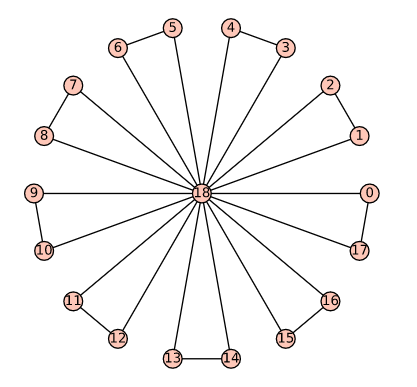
\includegraphics[scale=0.7]{clustering_graph.png}
\caption{Primer omrežja, kjer dve različni meri konvergirata h 0 in 1.}
\label{clustering_graph}
\end{center}
\end{figure}

$ C $ se v primeru zgornjega grafa manjša, saj število trikotnikov v grafu narašča veliko počasneje kot število vseh trojčkov vozlišč, ki so med sabo povezani.

$\langle C \rangle$ v grafu konvergira h 1, saj z vsako novo vejo dodamo 2 novi vozlišči, ki imata povezane vse svoje sosede.


\subsection{Effective diameter evolution}

Tabela \ref{tbg} prikazuje rezultate za posamezna omrežja. Rezultati za premer niso presenetljivi, saj se običajno z dodajanjem novih povezav (vsako leto dodamo nove povezave) in večanjem povprečnje stopnje vozlišč, zmanjšuje tudi najkrajša pot med vozlišči kar posledično vpliva na premer. 

\begin{table}[]
\centering
\caption{Podatki grafov}
\label{tbg}
\begin{tabular}{|l|l|l|l|}
\hline
 & Diameter & Number of nodes  & Average degree \\ \hline
10-11 & 27 & 18985 & 4.36945 \\ \hline
10-12 & 23 & 38356 & 5.73016 \\ \hline
10-13 & 21 & 56473 & 7.09553 \\ \hline
\end{tabular}
\end{table}


Psevdokoda:

Algoritem za iskanje $E_{90}$ je zelo preprost, saj je edini dodatni pogoj ta, da v BFS dodamo pogoj, kdaj naj se iskanje ustavi.

\begin{lstlisting}
za vsako vozlisce i v N
	dodaj i v vrsto
	dokler (vrsta ni prazna ALI ni preiskanih 90 odstotkov vozlisc)
		izvajaj obicajen BFS in izracunaj najdalso razdaljo 
	
	
\end{lstlisting}

\begin{lstlisting}
def BFS(G, node):
    D = dict()
    Q = Queue()
    Q.put(node)
    D[node] = 0
    while not Q.empty():
        i = Q.get()
        for j in G.neighbors(i):
            if j not in D and len(D)<0.9*G.number_of_nodes():
                D[j] = D[i] + 1
                Q.put(j)
    return D

def diameter(G):
    max_d = 0
    for n in G.nodes():
        max_d = max(max_d, np.max([y for x,y in  BFS(G, n).items()]))
    return max_d
\end{lstlisting}


\section{Graph models }

\subsection{Random node selection}

Če predpostavimo, da imamo že sestavljen graf, ki je predstavljen kot seznam povezav, potem je vzorčenje vozlišč z verjetnostjo $\frac{k_i}{2m}$ precej preprosto. Iz grafa izberemo naključno povezavo in nato še enkrat naključno izberemo enega izmed vozlišč, te povezave.

Psevdokoda:
        
\begin{lstlisting}
def get_random_edge(G):
	v_i,v_j = G.random_edge() #Operacija O(1)
	if random_bool:
		return v_i
	else:
		return v_j
\end{lstlisting}

Algoritem izbira naključne povezave, zato so vozlišča z večjo stopnjo izbrana z večjo verjetnostjo. Ko izberemo povezavo, je potrebno izbrati le še enega od vozlišč, ki jih povezava združuje. S tem smo vsako vozlišče izbrali z verjetnostjo $\frac{k_i}{2m}$.

\subsection{Node linking probability}

Pričakovana vrednost stopnje posameznega vozlišča $\Aver{k_i}$ je
\[\Aver{k_i} = \sum_{j \neq i} v_i v_j = v_i\sum_{j \neq i}v_j\]

Kar je v primeru $n\to\infty$ pribljižno enako:

\[\Aver{k_i} \approx v_i\sum_{j}v_j\]

Verjetnost povezave med vozlišči $p_{ij}$ lahko izračunamo iz stopenj vozlišč $\{k_1, k_2, \cdots, k_n\}$ na način:

\[p_{ij} = \frac{k_ik_j}{\sum_h k_h}\]

Enačba izhaja iz tega, da je povezava med dvema naključnima deloma povezave (angl. stub) enaka $\frac{1}{\sum_h k_h}$. To vrednost nato le še pomnožimo z $k_i$ in $k_j$, ki predstavljata število teh stub-ov izven vozlišč $i$ in $j$.

\subsection{Node degree distributions }



\begin{figure}[htbp]
\begin{center}
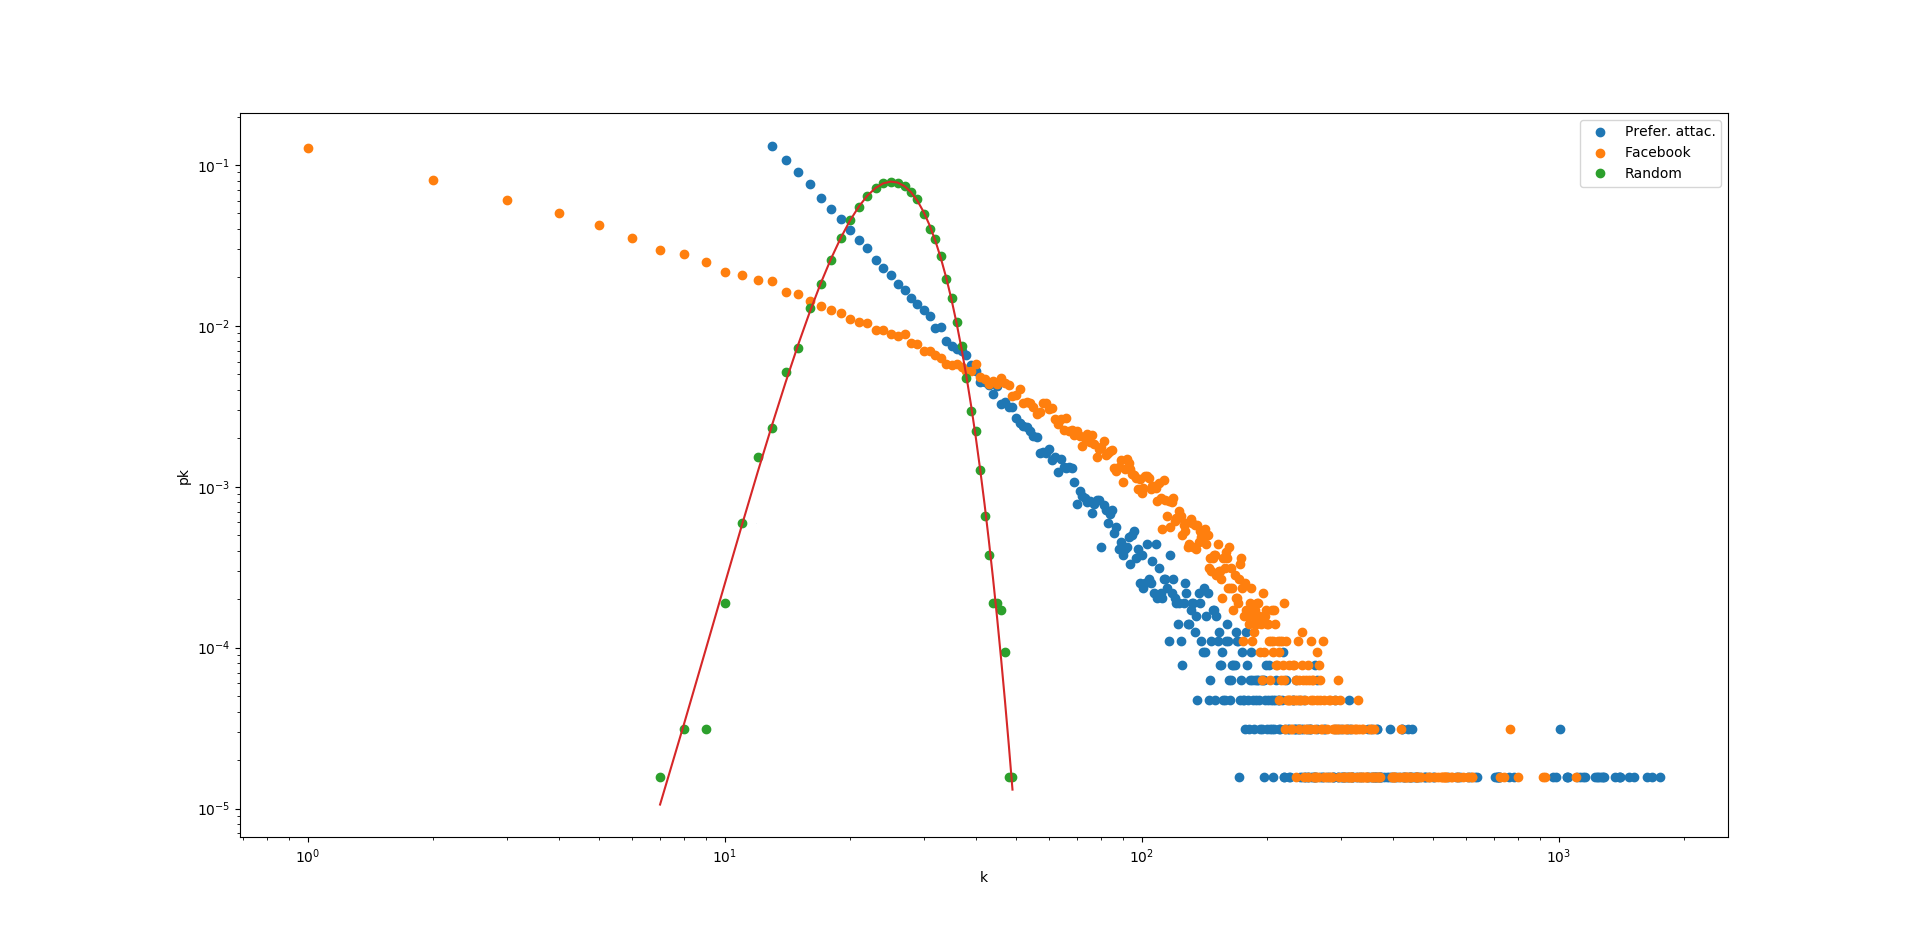
\includegraphics[scale=0.27]{distr.png}
\caption{Distribucija vozlišč za različna omrežja.}
\label{distr}
\end{center}
\end{figure}

Slika \ref{distr} prikazuje porazdelitve stopenj vozlišč za različna omrežja. Razvidno je, da je ustvarjen Erdos-Renyi graf enak distribuciji, ki bi jo pričakovali in je narisana s črto. Drugi dve distribuciji sta še distribucija Facebook omrežja in preferential attachment distribucija, ki se od naključnega omrežja zelo razlikujeta.




\begin{minipage}{\linewidth}

Gradnja grafa:

\begin{lstlisting}
def build_graph(n, k):
    l = []
    
    #Fully connected
    for i in range(np.math.ceil(k)+1):
        for j in range(np.math.ceil(k)+1):
            if i<j:
                l.append((i,j))
                
    #Other nodes       
    for h in range(n - np.math.ceil(k) - 1):
        for x,y in random.sample(l, np.math.ceil(k/2)):
           if bool(random.getrandbits(1)):
               l.append(("n"+str(h), x))
           else:
               l.append(("n" + str(h), y))

    G = nx.Graph()
    for x,y in l:
        G.add_edge(x, y)
    return G
\end{lstlisting}
\end{minipage}


\begin{minipage}{\linewidth}
Izračun pk:

\begin{lstlisting}
c = collections.Counter([y for x,y in G.degree()])
k_avg = np.mean([y for x,y in G.degree()])
c1_ = np.array([f for k,f in c.items()])
plt.plot([k for k,f in c.items()],c1_/np.sum(c1_), 'o', label='Facebook')
\end{lstlisting}
\end{minipage}

\section{Node position}

Tabela \ref{cor_t} prikazuje Pearsonovo korelacijo med številom avtov v posameznem vozlišču in merami, ki jih vrnejo različni postopki za ugotavljanje pomembnosti vozlišč. Najslabša je bila mera Node clustering coef., saj se v celotnem omrežju ne pojavi noben trikotnik, zato je mera vedno 0. 

\begin{table}[]
\centering
\caption{Korelacije med dejanskimi vrednostmi in izračunanimi značilkami}
\label{cor_t}
\begin{tabular}{|l|l|}
\hline
Algoritem & Korelacija   \\ \hline
Node clus.
coeff. & 0   \\ \hline
Node degree & 0.27571  \\ \hline
Closeness centr.  &  0.61918  \\ \hline
Between. centr.  & 0.62257  \\ \hline
Pagerank  &  0.11971 \\ \hline
\end{tabular}
\end{table} 

Največjo korelacijo z resničnim pretokom ima mera Betweenness centrality, kar je pričakovano, saj merimo število poti, ki gredo skozi vozlišče. Podatki o tej meri so prikazani v tabeli \ref{bc}

\begin{table}[]
\centering
\caption{Najboljša vozlišča glede na Betweenness centrality}
\label{bc}
\begin{tabular}{|l|l|l|}
\hline
Ime & Centrality & Pretok   \\ \hline
Zadobrova& 0.4991 &   33779 \\ \hline
Sneberje & 0.4798 &  20686  \\ \hline
Šentjakob & 0.4760 &  26423  \\ \hline
Domžale & 0.4720 &  26423  \\ \hline
Krtina & 0.4678 &  20686  \\ \hline
Lukovica & 0.4632 &  19177  \\ \hline
Blagovica & 0.4584 &  37784  \\ \hline
Trojane & 0.4534 &  36066  \\ \hline
Vransko & 0.4480 &  35547  \\ \hline
Šentrupert & 0.4424 &  18088  \\ \hline
\end{tabular}
\end{table}

\begin{minipage}{\linewidth}

Koda:

\begin{lstlisting}
G = nx.read_adjlist("path")

def read_real_values():
    with open("path", encoding="UTF-8") as f:
        lines = [x.strip() for x in f.readlines() if x.startswith("#")]
        for l in lines:
            h = l.split("\"")
            yield h[0][1:].strip(), float(h[2].strip())

vals = list(read_real_values())

c1 = [(int(x),y) for x,y in nx.clustering(G).items()]
c1.sort()


c2 = [(int(x), y) for x,y in nx.degree(G)]
c2.sort()


c3 = [(int(x), y) for x,y in nx.closeness_centrality(G).items()]
c3.sort()


c4 = [(int(x), y) for x,y in nx.betweenness_centrality(G).items()]
c4.sort()


c5 = [(int(x), y) for x,y in nx.pagerank(G).items()]
c5.sort()




c2_cor = np.corrcoef([y for x,y in vals], [y for x,y in c2])[0,1]
c3_cor = np.corrcoef([y for x,y in vals], [y for x,y in c3])[0,1]
c4_cor = np.corrcoef([y for x,y in vals], [y for x,y in c4])[0,1]
c5_cor = np.corrcoef([y for x,y in vals], [y for x,y in c5])[0,1]

print(c2_cor)
print(c3_cor)
print(c4_cor)
print(c5_cor)
\end{lstlisting}
\end{minipage}


\end{document}
